\documentclass{beamer}
\usepackage{../tut-slides}
\usepackage{../mathoperatorsAuD}

\usepackage{amsmath,amssymb}
\usepackage{stmaryrd}
\usepackage{enumerate}
%\usepackage[inline]{enumitem} 		%customize label
%\newcommand{\labelitemi}{\raisebox{1pt}{\scalebox{.9}{$\blacktriangleright$}}}
%\newcommand{\labelitemii}{$\vartriangleright$}
%\newcommand{\labelitemiii}{--}
\setbeamertemplate{itemize item}{\raisebox{1pt}{\scalebox{.9}{$\blacktriangleright$}}}
\setbeamertemplate{itemize subitem}{$\vartriangleright$}

\usepackage{booktabs}
\usepackage{tabularx}
\usepackage{tabu}
\newcommand*\head{\rowfont{\bfseries}}
\newcommand*{\tw}{\rowfont{\ttfamily}}
\renewcommand{\tabularxcolumn}[1]{>{\hspace{0pt}}m{#1}}

\usepackage{cancel}

%%%% EBNF-Terme %%%%
\newcommand{\wdh}[1]{\hat{\{} \ #1 \ \hat{\}}}
\newcommand{\opt}[2]{\hat{(} \ #1 \ \hat{|} \ #2 \ \hat{)}}
\newcommand{\byp}[1]{\hat{[} \ #1 \ \hat{]}}
\newcommand{\rdb}[1]{\hat{(} \ #1 \ \hat{)}}

\newcommand{\sem}[1]{\left\llbracket #1 \right\rrbracket}


\begin{document}	
	\title{Algorithmen und Datenstrukturen}
	\subtitle{Übung 3: Extended Backus-Naur-Form}
	\author{Eric Kunze}
	\email{eric.kunze@mailbox.tu-dresden.de}
	\city{TU Dresden}
%	\institute{Lehrstuhl für Grundlagen der Programmierung}
	\titlegraphic{
\includegraphics[width=2cm]{../TUD-white.pdf}}
	\date{07.11.2019}

	\maketitle


%%%%%%%%%%%%%%%%%%%%%%%%%%%%%%%%%%%%%%%%%%%%%%%%%%%%%%%%%%%%%%%%%%%%%%%%%%%%%

\begin{frame} \frametitle{EBNF-Definition}
	\small
	\begin{itemize}
		\item EBNF-Definition besteht aus endlicher Menge von EBNF-Regeln.
		\item Jede EBNF-Regel besteht aus einer linken und einer rechten Seite, die rechte Seite ist ein EBNF-Term.
	\end{itemize}
	\pause
	\begin{block}{Definition: EBNF-Term}
		Seien $V$ eine endliche Menge (syntaktische Variablen) und $\Sigma$ eine endliche Menge (Terminalsymbole) mit $V \cap \Sigma = \emptyset$. Die Menge der EBNF-Terme über $V$ und $\Sigma$ (notiere: $T(\Sigma, V)$), ist die kleinste Menge $T \subseteq \brackets{V \cup \Sigma \cup \menge{\hat{\{}, \hat{\}}, \hat{[}, \hat{]}, \hat{(}, \hat{)}, \hat{|}}}$ mit $V \subseteq T$, $\Sigma \subseteq T$ und
		\begin{itemize}
			\item Wenn $\alpha \in T$, so auch $\rdb{\alpha} \in T$, $\wdh{\alpha} \in T$, $\byp{\alpha} \in T$.
			\item Wenn $\alpha_1, \alpha_2 \in T$, so auch $\opt{\alpha_1}{\alpha_2} \in T$, $\alpha_1 \alpha_2 \in T$
		\end{itemize}
	\end{block}
\end{frame}

\begin{frame} \frametitle{Übersetzung Syntaxdiagramme $\leftrightarrow$ EBNF}
	\centering
	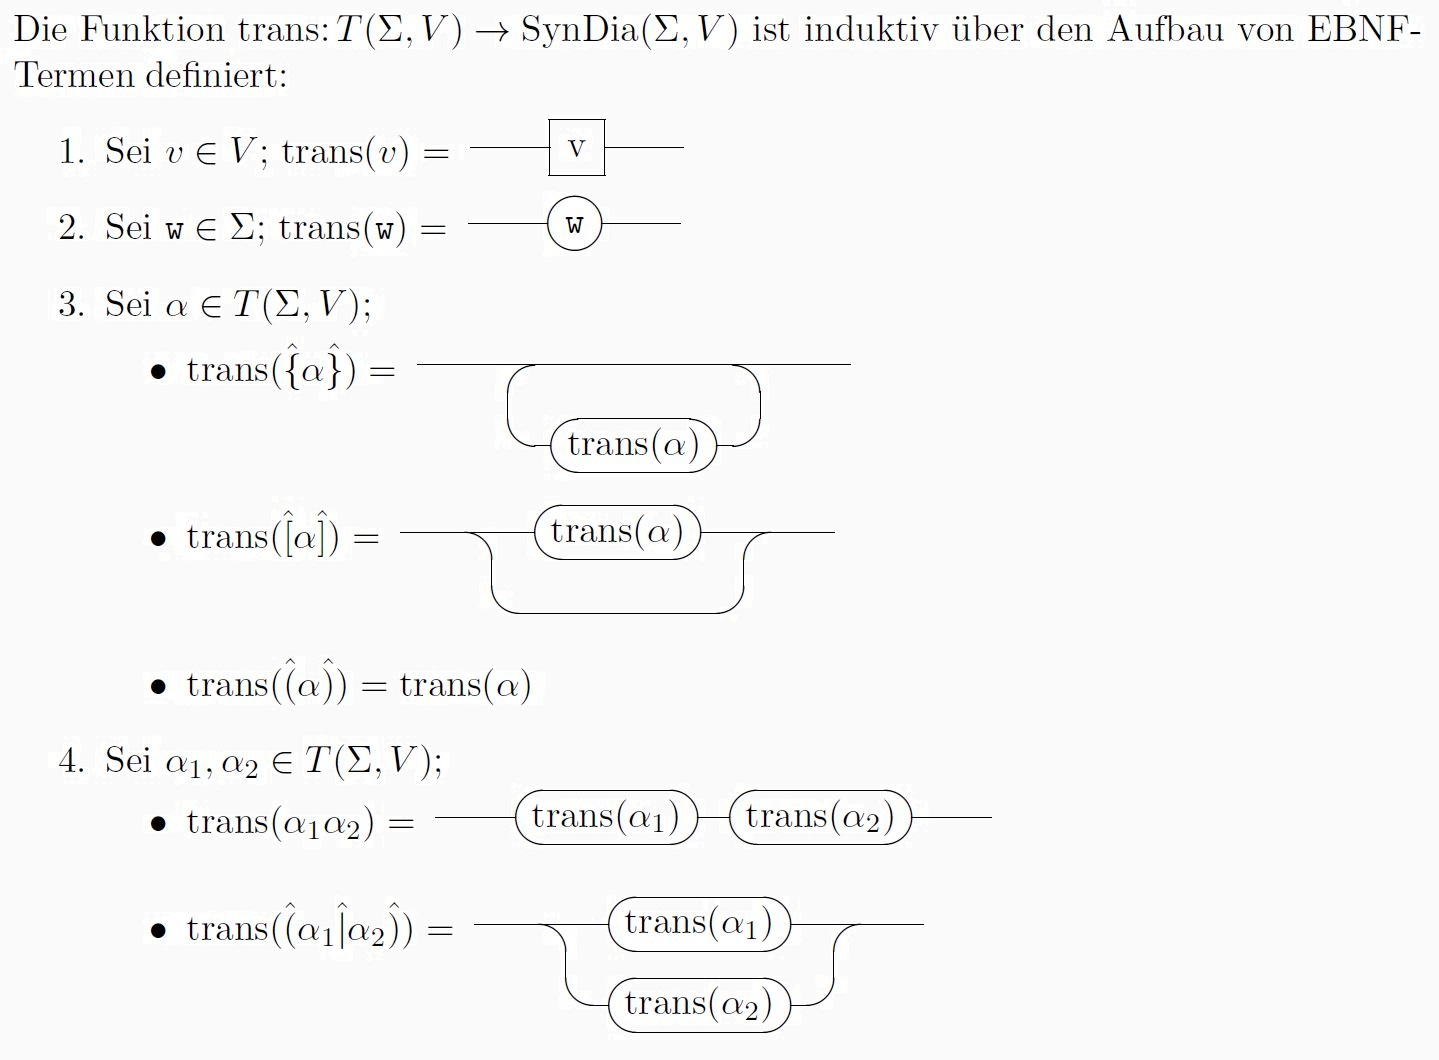
\includegraphics[width=.9\textwidth]{tut03_trans.jpg}
\end{frame}

\begin{frame} \frametitle{Semantik von EBNF-Termen}
	\begin{itemize}
		\item Sei $\mathcal{E} = (V,\Sigma,S,R)$ eine EBNF-Definition.
		\item $v \in V \leadsto W(\mathcal{E},v) = \rho(v)$ (syntaktische Kategorie)
		\item Semantik $\abb{\sem{\cdot}}{\underbrace{T(\Sigma, V)}_{\alpha}}{((\underbrace{V \to \pows{\Sigma^\ast}}_{\rho}) \to \pows{\Sigma^\ast})}$
		\item[] 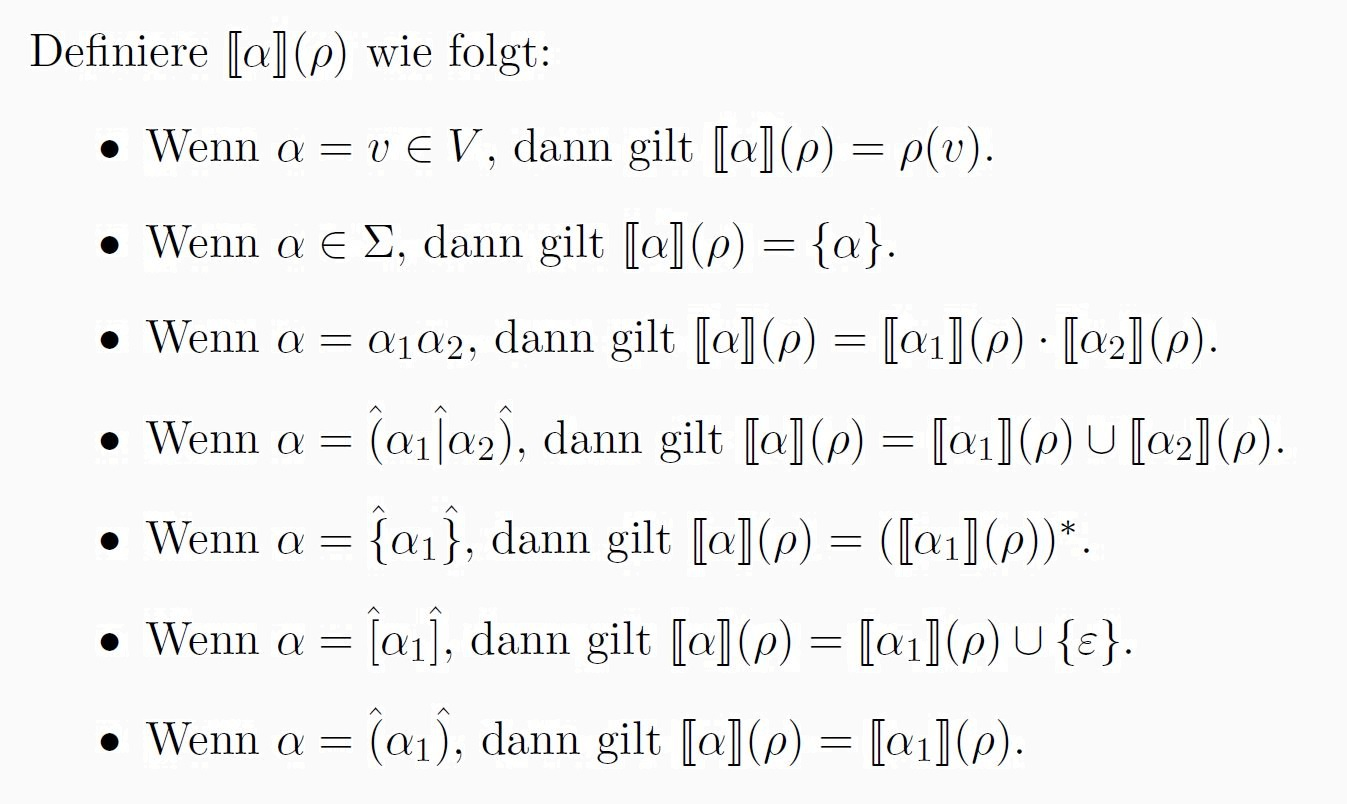
\includegraphics[width=.9\textwidth]{tut03_semantik.jpg}
	\end{itemize}	
\end{frame}

\section{Übungsblatt 3}

\begin{frame} \frametitle{Aufgabe 1 --- Teil (a)}
	Sei $\Sigma = \menge{a,b}$.
	\begin{align*}
		L &= \menge{a^n b^m v a w \mid n \ge m \ge 0, v,w \in \Sigma^\ast \mit \abs{v} = \abs{w}} \\
		&= \menge{a^n a^m b^n \mid m,n \in \N} * \left[\bigcup_{n \in \N} \menge{a,b}^n * \menge{a} * \menge{a,b}^n \right]
	\end{align*}
	
	\begin{center}
		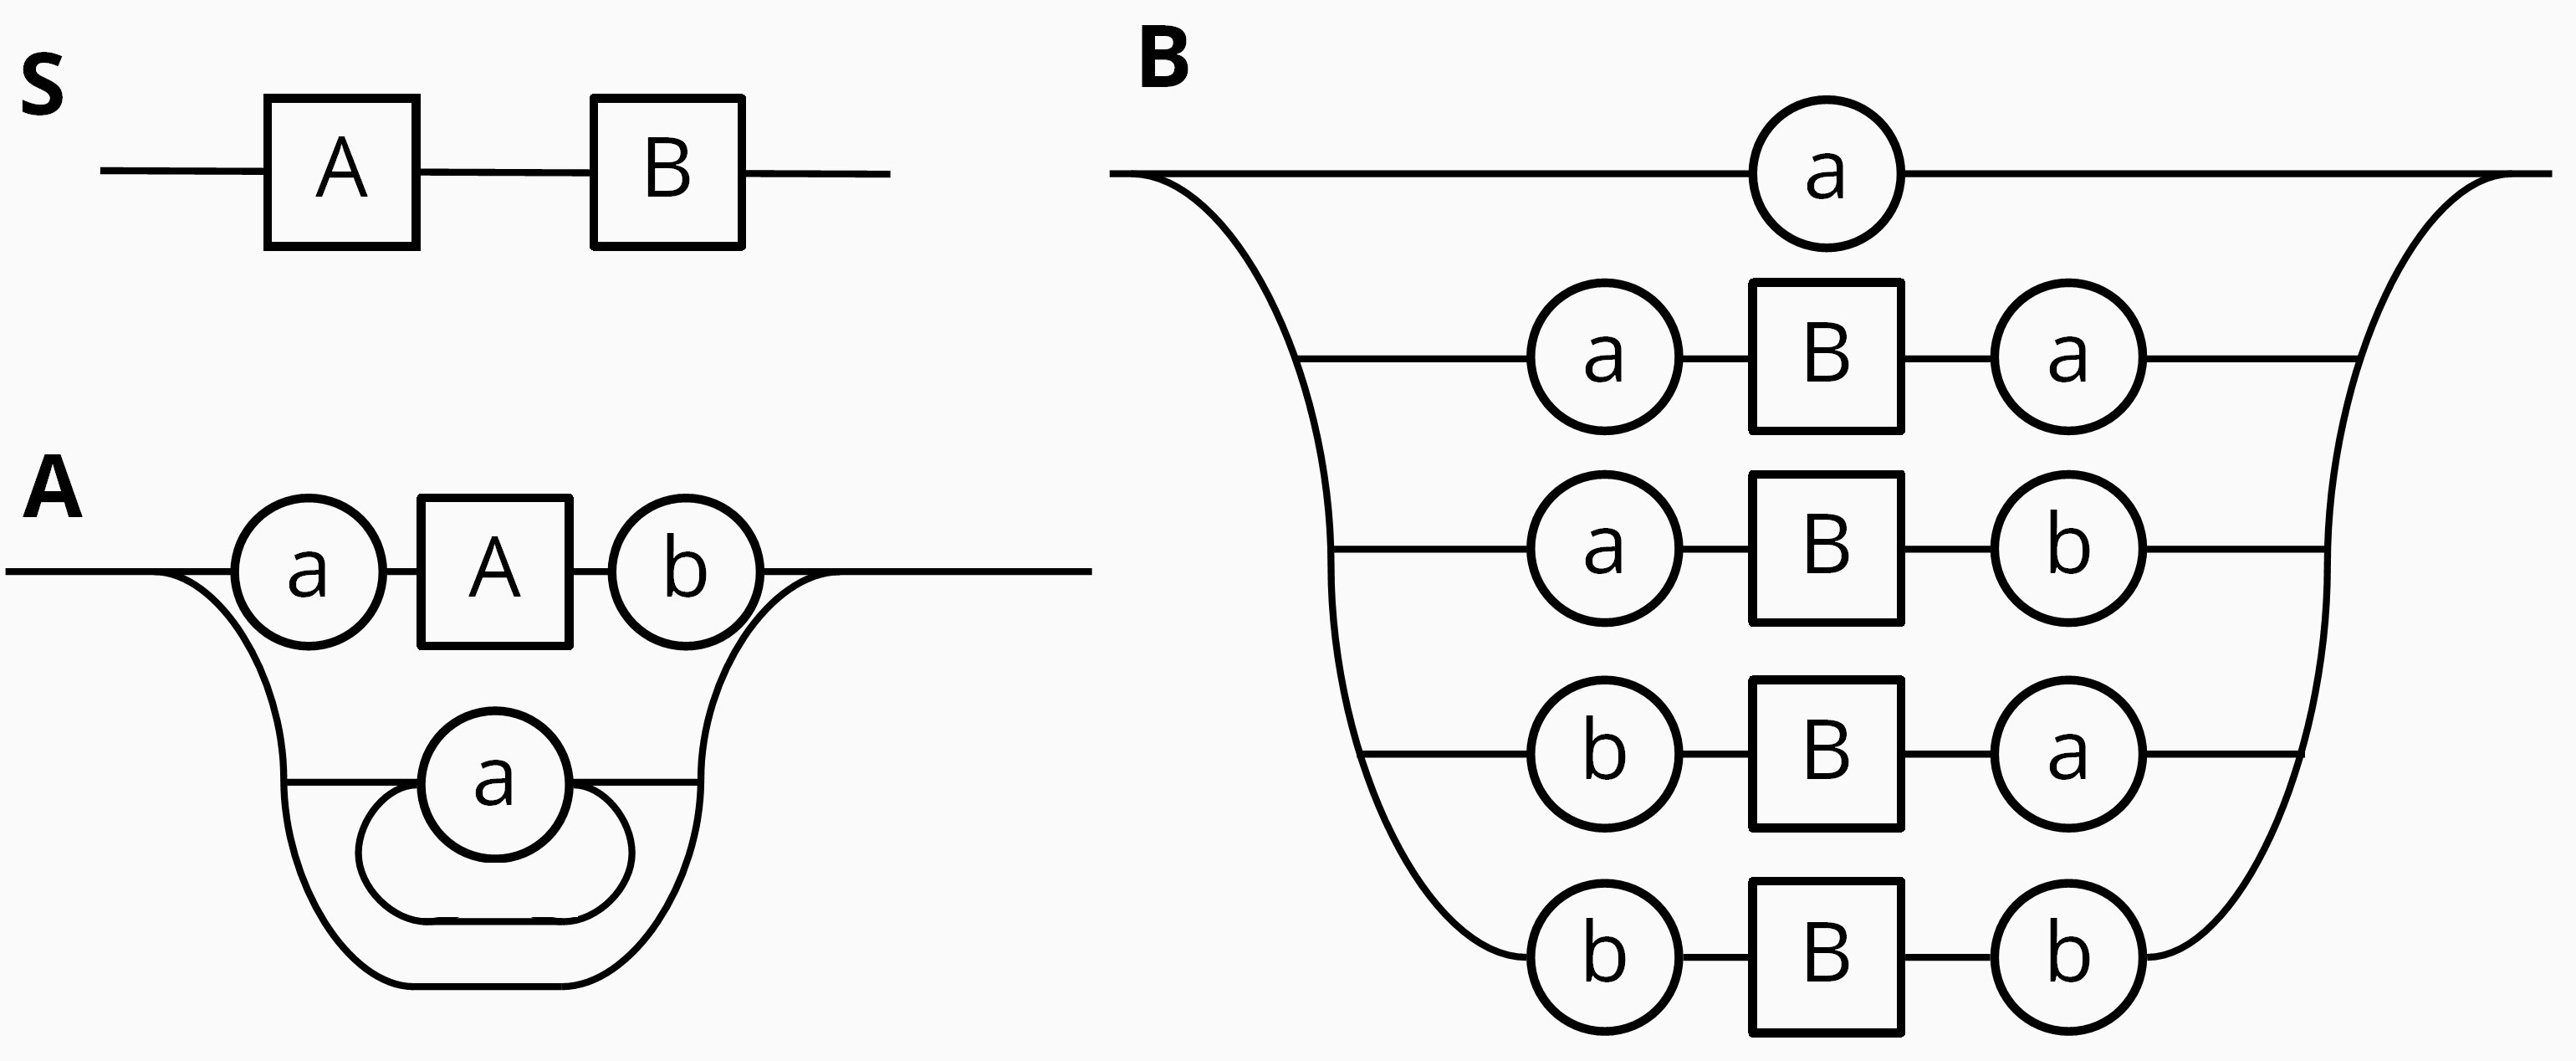
\includegraphics[width=\textwidth]{tut03_syntax_dia_1a.jpg}
	\end{center}
\end{frame}

\begin{frame} \frametitle{Aufgabe 1 --- Teil (b)}
	\centering
	\begin{tabular}{l|r}
		Wort & Markenkeller \\ \hline
		$\epsilon$ & $1$ \\
		a & $31$ \\
		aa & $\cancel{3}1$ \\
		aab & $\cancel{1}$ \\
		aab & $2$ \\
		aaba & $52$ \\
		aabab & $752$ \\
		aababa & $\cancel{7}52$ \\
		aababab & $\cancel{5}2$ \\
		aabababb & $\cancel{2}$ \\
		aabababb & --
	\end{tabular}
\end{frame}

\begin{frame} \frametitle{Aufgabe 2}
	\begin{center}
		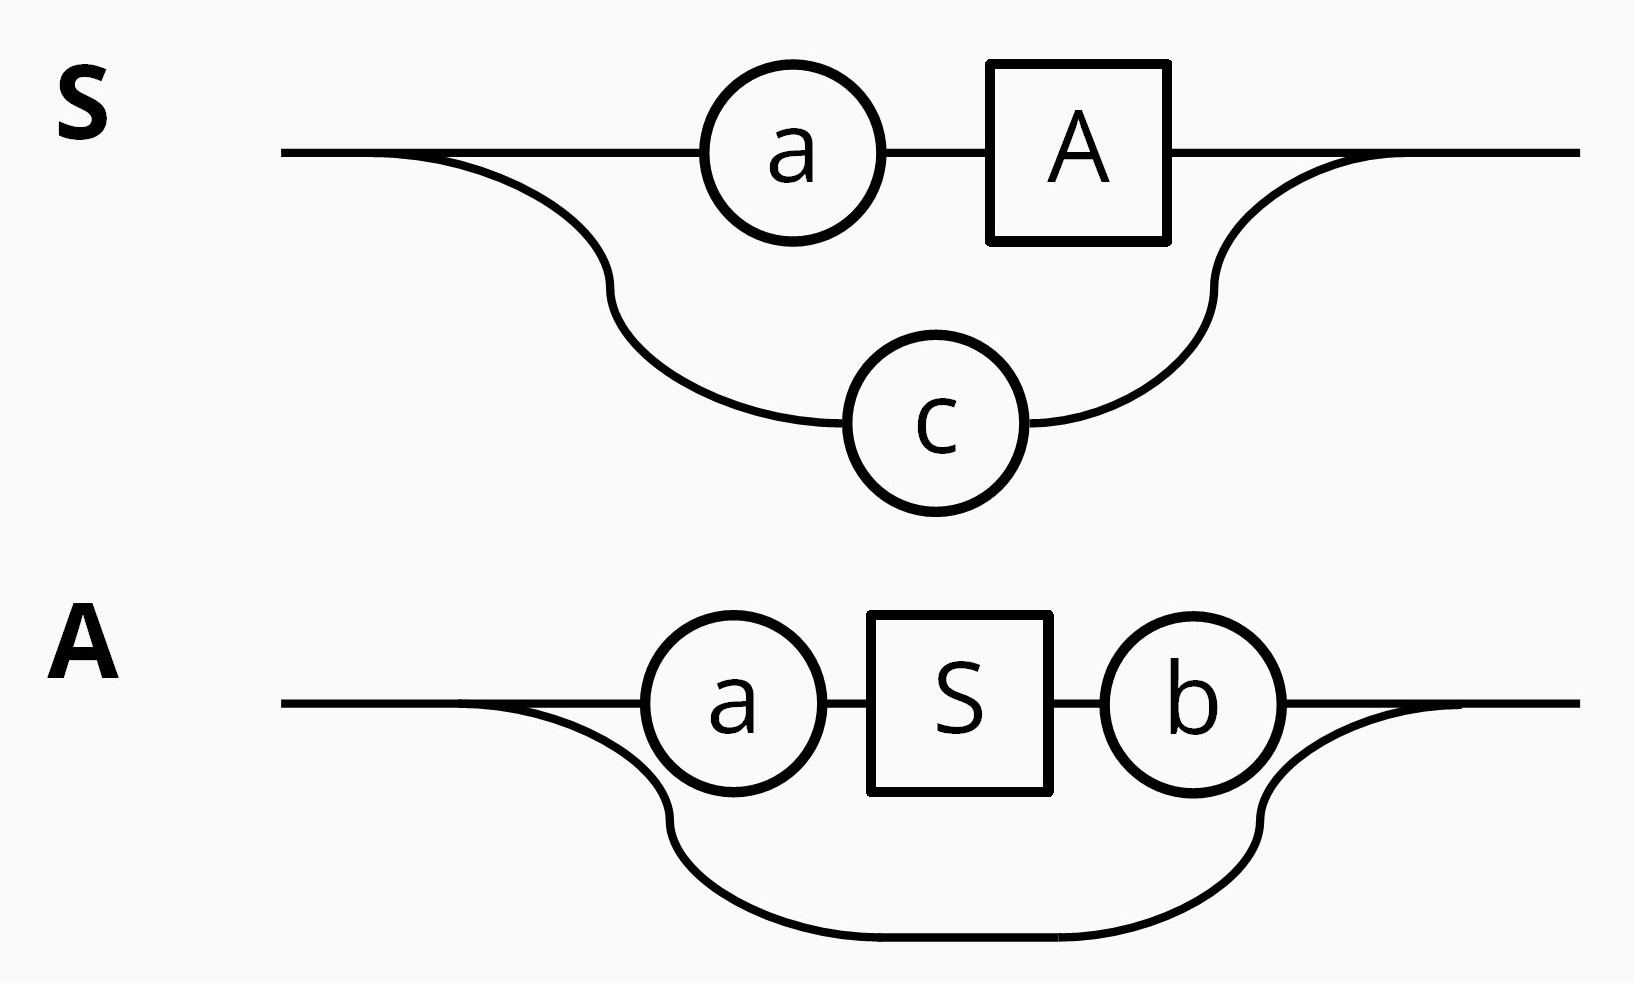
\includegraphics[width=.5\textwidth]{tut03_syntax_dia_2a.jpg}
	\end{center}

	\begin{equation*}
		W(\mathcal{E},S) = \menge{a^{2n} x b^n \mid x \in \menge{a,c}, n \ge 0}
	\end{equation*}
\end{frame}

\begin{frame} \frametitle{Aufgabe 3 --- Teil (a)}
	Sei $\Sigma = \menge{a,b}$ und eine EBNF-Definition $\mathcal{E} = (V,\Sigma,S,R)$ mit 
	\begin{equation*}
		W(\mathcal{E}) = \menge{a^i b^{2n} a^j b^{3n} a^k \mid i,j,k \ge 2, n \ge 0} 
	\end{equation*}
	gegeben. \pause
	\begin{align*}
		V &= \menge{S,A,B} \\
		R &= \menge{S ::= ABA , A ::= aa \ \wdh{a}, B ::= \opt{bbBbbb}{A}}
	\end{align*}
\end{frame}

\begin{frame} \frametitle{Aufgabe 3 --- Teil (b)}
	$\mathcal{E} = (V,\Sigma,S,R)$, $V = \menge{S}$, $\Sigma = \menge{a,b}$, $R = \menge{S ::= \opt{aSa}{\byp{b}}}$. 
	
	Zu zeigen: $W(\mathcal{E},S) = \menge{a^n w a^n \mid n \ge 0, w \in \menge{\epsilon,b}}$.
	
	\pause 
	
	\begin{align*}
		\sem{\opt{aSa}{\byp{b}}}(\rho) 
		&= \sem{aSa}(\rho) \cup \sem{\byp{b}}(\rho) \\
		&= \sem{a}(\rho) * \sem{S}(\rho) * \sem{a}(\rho) \cup \brackets{\sem{b}(\rho) \cup \menge{\epsilon}} \\
		&= \menge{a} * \rho(S) * \menge{a} \cup \brackets{\menge{b} \cup \menge{\epsilon}} \\
		&= \menge{a^n w a^n \mid n \ge 1, w \in \menge{\epsilon, b}} \cup \menge{\epsilon,b} \\
		&= \rho(S)
	\end{align*}
\end{frame}

\begin{frame} \frametitle{Aufgabe 4 --- Teil (a)}
	$W(\mathcal{E},S) = \menge{a^{n+m} w b^\ell a^n \mid n,m \ge 0, 0 \le \ell \le m, w \in \Sigma^\ast}$
	\pause
	\begin{align*}
		V = \menge{S,A,B} \quad \und \quad  
		R = \Big\{ S &::= \opt{aSa}{A} ,\\
			A & ::= \opt{aA \byp{b}}{B}, \\
			B & ::= \wdh{\opt{a}{b}} \quad \Big\}
	\end{align*}
\end{frame}

\begin{frame} \frametitle{Aufgabe 4 --- Teil (b)}
	\begin{align*}
		f(\rho) = \begin{pmatrix} f(\rho)(S) \\ f(\rho)(A) \end{pmatrix} 
		= \begin{pmatrix} \sem{\byp{aAb}}(\rho) \\ \sem{\opt{Sc}{cS}}(\rho) \end{pmatrix} 
		= \begin{pmatrix}
		\menge{a} * \rho(A) * \menge{b} \\ \rho(S) * \menge{c} \cup \menge{c} * \rho(S)
		\end{pmatrix}
	\end{align*}
	\begin{align*}
		\begin{pmatrix} \emptyset \\ \emptyset \end{pmatrix}
		\mapsto
		\begin{pmatrix} \menge{\epsilon} \\ \emptyset \end{pmatrix}
		\mapsto
		\begin{pmatrix} \menge{\epsilon} \\ \menge{c} \end{pmatrix}
		&\mapsto
		\begin{pmatrix} \menge{\epsilon,acb} \\ \menge{c} \end{pmatrix} \\
		&\mapsto
		\begin{pmatrix} \menge{\epsilon,acb} \\ \menge{c,acbc,cacb} \end{pmatrix} \\
		&\mapsto
		\begin{pmatrix} \menge{\epsilon,acb,aacbcb,acacbb} \\ \menge{c,acbc,cacb} \end{pmatrix}
	\end{align*}
\end{frame}

\begin{frame} \frametitle{Aufgabe 4 --- Teil (c)}
	\centering
	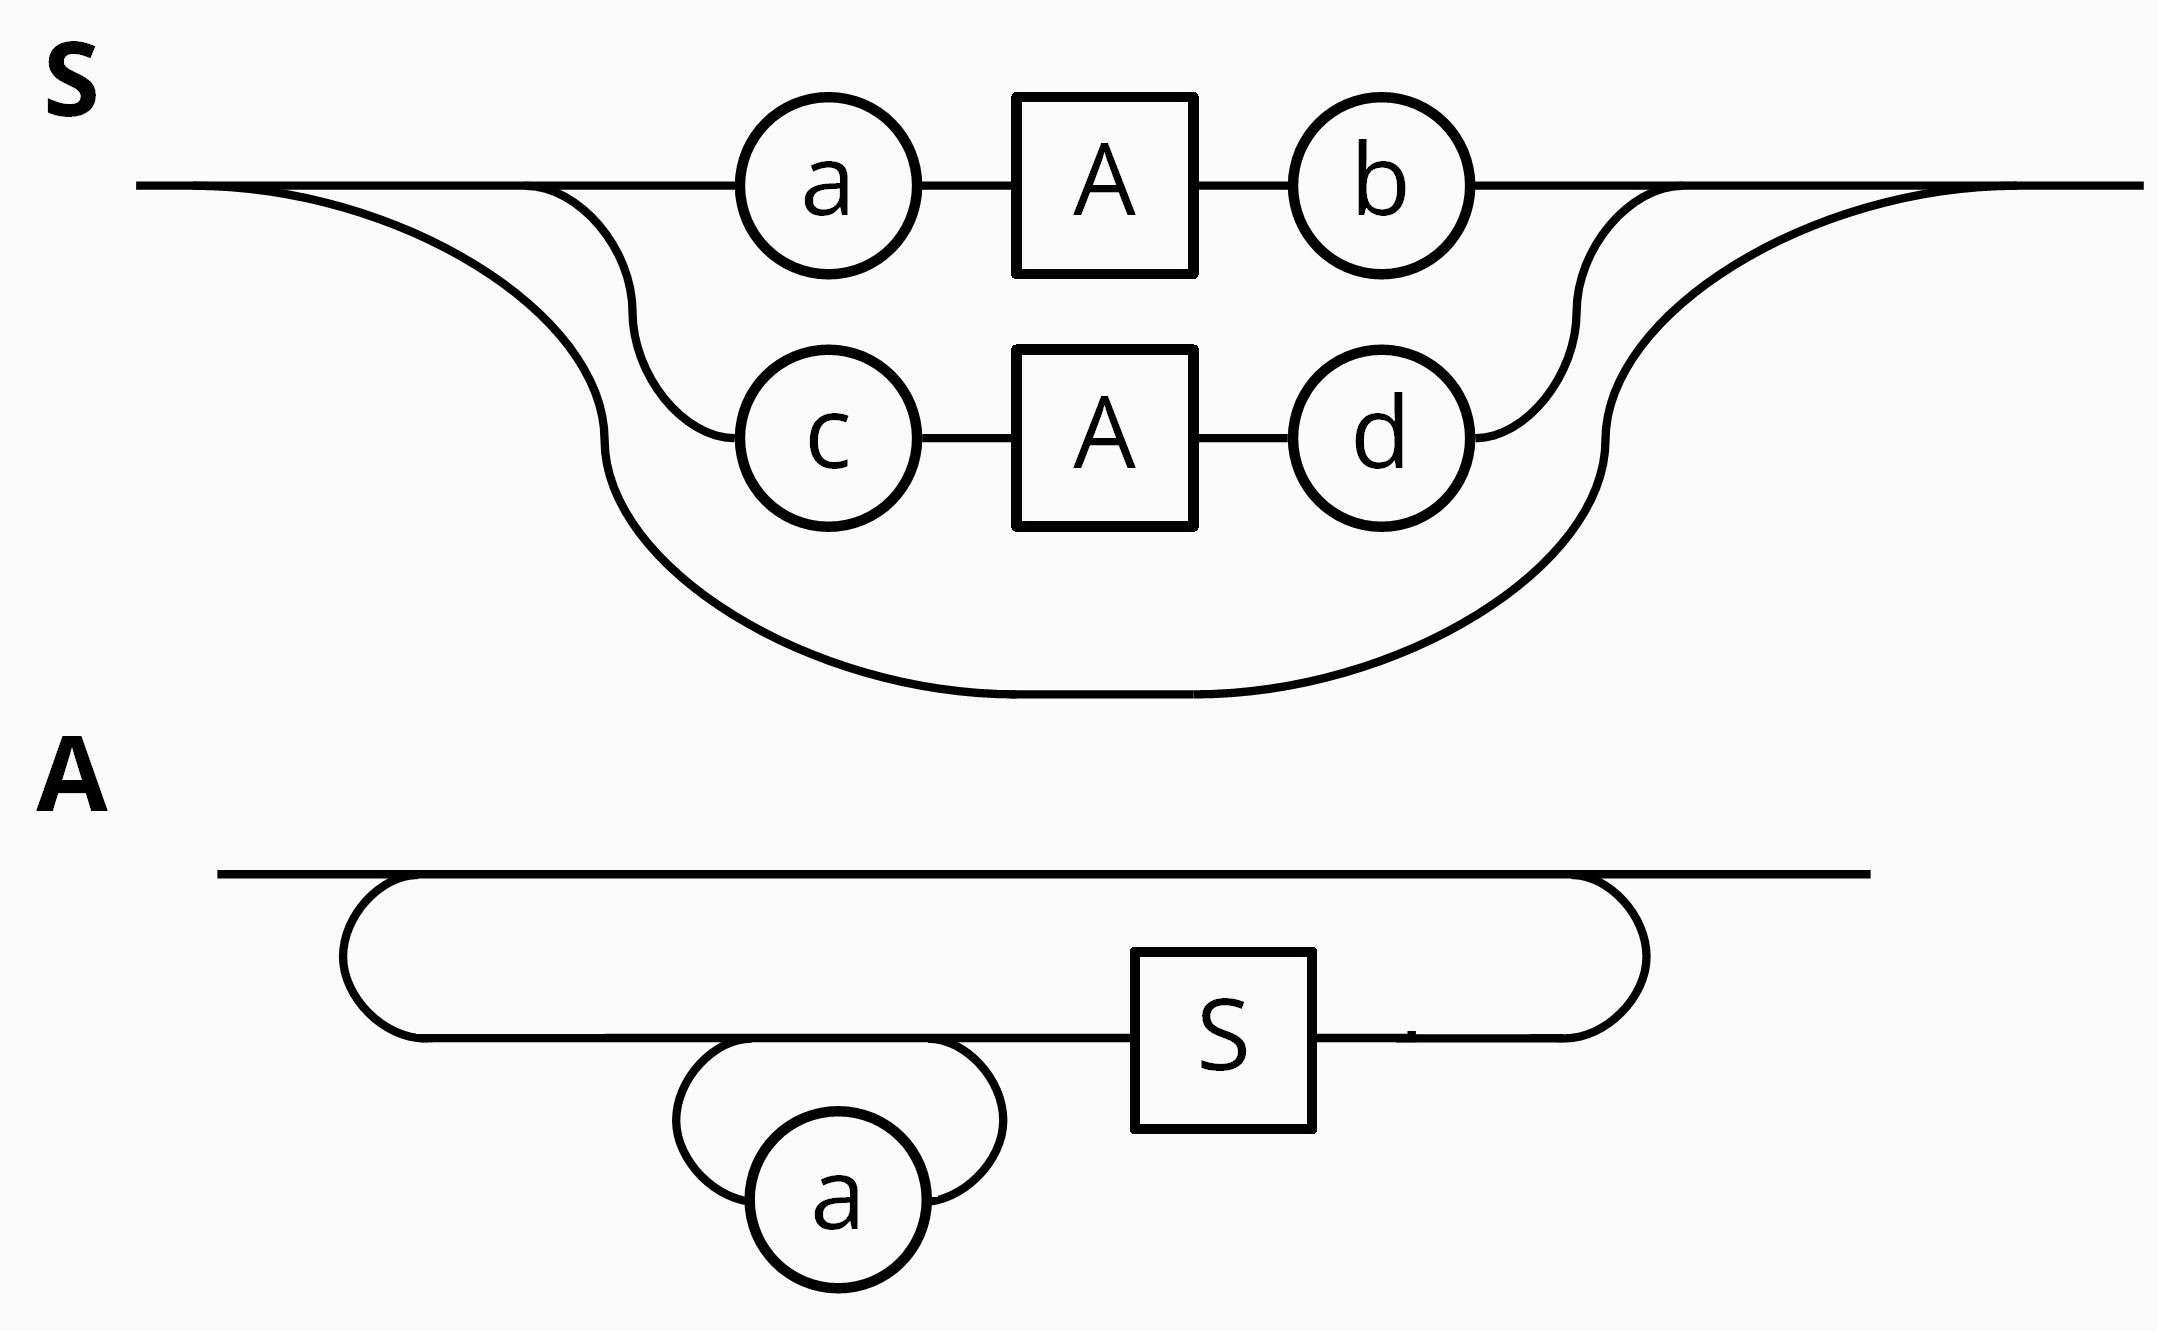
\includegraphics[width=\textwidth]{tut03_syntax_dia_4c.jpg}
\end{frame}


\end{document}